% Options for packages loaded elsewhere
\PassOptionsToPackage{unicode}{hyperref}
\PassOptionsToPackage{hyphens}{url}
%
\documentclass[
  11pt,
  ignorenonframetext,
]{beamer}
\usepackage{pgfpages}
\setbeamertemplate{caption}[numbered]
\setbeamertemplate{caption label separator}{: }
\setbeamercolor{caption name}{fg=normal text.fg}
\beamertemplatenavigationsymbolsempty
% Prevent slide breaks in the middle of a paragraph
\widowpenalties 1 10000
\raggedbottom
\setbeamertemplate{part page}{
  \centering
  \begin{beamercolorbox}[sep=16pt,center]{part title}
    \usebeamerfont{part title}\insertpart\par
  \end{beamercolorbox}
}
\setbeamertemplate{section page}{
  \centering
  \begin{beamercolorbox}[sep=12pt,center]{part title}
    \usebeamerfont{section title}\insertsection\par
  \end{beamercolorbox}
}
\setbeamertemplate{subsection page}{
  \centering
  \begin{beamercolorbox}[sep=8pt,center]{part title}
    \usebeamerfont{subsection title}\insertsubsection\par
  \end{beamercolorbox}
}
\AtBeginPart{
  \frame{\partpage}
}
\AtBeginSection{
  \ifbibliography
  \else
    \frame{\sectionpage}
  \fi
}
\AtBeginSubsection{
  \frame{\subsectionpage}
}
\usepackage{amsmath,amssymb}
\usepackage{lmodern}
\usepackage{iftex}
\ifPDFTeX
  \usepackage[T1]{fontenc}
  \usepackage[utf8]{inputenc}
  \usepackage{textcomp} % provide euro and other symbols
\else % if luatex or xetex
  \usepackage{unicode-math}
  \defaultfontfeatures{Scale=MatchLowercase}
  \defaultfontfeatures[\rmfamily]{Ligatures=TeX,Scale=1}
\fi
\usetheme[]{metropolis}
% Use upquote if available, for straight quotes in verbatim environments
\IfFileExists{upquote.sty}{\usepackage{upquote}}{}
\IfFileExists{microtype.sty}{% use microtype if available
  \usepackage[]{microtype}
  \UseMicrotypeSet[protrusion]{basicmath} % disable protrusion for tt fonts
}{}
\makeatletter
\@ifundefined{KOMAClassName}{% if non-KOMA class
  \IfFileExists{parskip.sty}{%
    \usepackage{parskip}
  }{% else
    \setlength{\parindent}{0pt}
    \setlength{\parskip}{6pt plus 2pt minus 1pt}}
}{% if KOMA class
  \KOMAoptions{parskip=half}}
\makeatother
\usepackage{xcolor}
\newif\ifbibliography
\usepackage{color}
\usepackage{fancyvrb}
\newcommand{\VerbBar}{|}
\newcommand{\VERB}{\Verb[commandchars=\\\{\}]}
\DefineVerbatimEnvironment{Highlighting}{Verbatim}{commandchars=\\\{\}}
% Add ',fontsize=\small' for more characters per line
\newenvironment{Shaded}{}{}
\newcommand{\AlertTok}[1]{\textcolor[rgb]{1.00,0.00,0.00}{\textbf{#1}}}
\newcommand{\AnnotationTok}[1]{\textcolor[rgb]{0.38,0.63,0.69}{\textbf{\textit{#1}}}}
\newcommand{\AttributeTok}[1]{\textcolor[rgb]{0.49,0.56,0.16}{#1}}
\newcommand{\BaseNTok}[1]{\textcolor[rgb]{0.25,0.63,0.44}{#1}}
\newcommand{\BuiltInTok}[1]{\textcolor[rgb]{0.00,0.50,0.00}{#1}}
\newcommand{\CharTok}[1]{\textcolor[rgb]{0.25,0.44,0.63}{#1}}
\newcommand{\CommentTok}[1]{\textcolor[rgb]{0.38,0.63,0.69}{\textit{#1}}}
\newcommand{\CommentVarTok}[1]{\textcolor[rgb]{0.38,0.63,0.69}{\textbf{\textit{#1}}}}
\newcommand{\ConstantTok}[1]{\textcolor[rgb]{0.53,0.00,0.00}{#1}}
\newcommand{\ControlFlowTok}[1]{\textcolor[rgb]{0.00,0.44,0.13}{\textbf{#1}}}
\newcommand{\DataTypeTok}[1]{\textcolor[rgb]{0.56,0.13,0.00}{#1}}
\newcommand{\DecValTok}[1]{\textcolor[rgb]{0.25,0.63,0.44}{#1}}
\newcommand{\DocumentationTok}[1]{\textcolor[rgb]{0.73,0.13,0.13}{\textit{#1}}}
\newcommand{\ErrorTok}[1]{\textcolor[rgb]{1.00,0.00,0.00}{\textbf{#1}}}
\newcommand{\ExtensionTok}[1]{#1}
\newcommand{\FloatTok}[1]{\textcolor[rgb]{0.25,0.63,0.44}{#1}}
\newcommand{\FunctionTok}[1]{\textcolor[rgb]{0.02,0.16,0.49}{#1}}
\newcommand{\ImportTok}[1]{\textcolor[rgb]{0.00,0.50,0.00}{\textbf{#1}}}
\newcommand{\InformationTok}[1]{\textcolor[rgb]{0.38,0.63,0.69}{\textbf{\textit{#1}}}}
\newcommand{\KeywordTok}[1]{\textcolor[rgb]{0.00,0.44,0.13}{\textbf{#1}}}
\newcommand{\NormalTok}[1]{#1}
\newcommand{\OperatorTok}[1]{\textcolor[rgb]{0.40,0.40,0.40}{#1}}
\newcommand{\OtherTok}[1]{\textcolor[rgb]{0.00,0.44,0.13}{#1}}
\newcommand{\PreprocessorTok}[1]{\textcolor[rgb]{0.74,0.48,0.00}{#1}}
\newcommand{\RegionMarkerTok}[1]{#1}
\newcommand{\SpecialCharTok}[1]{\textcolor[rgb]{0.25,0.44,0.63}{#1}}
\newcommand{\SpecialStringTok}[1]{\textcolor[rgb]{0.73,0.40,0.53}{#1}}
\newcommand{\StringTok}[1]{\textcolor[rgb]{0.25,0.44,0.63}{#1}}
\newcommand{\VariableTok}[1]{\textcolor[rgb]{0.10,0.09,0.49}{#1}}
\newcommand{\VerbatimStringTok}[1]{\textcolor[rgb]{0.25,0.44,0.63}{#1}}
\newcommand{\WarningTok}[1]{\textcolor[rgb]{0.38,0.63,0.69}{\textbf{\textit{#1}}}}
\usepackage{longtable,booktabs,array}
\usepackage{calc} % for calculating minipage widths
\usepackage{caption}
% Make caption package work with longtable
\makeatletter
\def\fnum@table{\tablename~\thetable}
\makeatother
\setlength{\emergencystretch}{3em} % prevent overfull lines
\providecommand{\tightlist}{%
  \setlength{\itemsep}{0pt}\setlength{\parskip}{0pt}}
\setcounter{secnumdepth}{-\maxdimen} % remove section numbering
\ifLuaTeX
  \usepackage{selnolig}  % disable illegal ligatures
\fi
\IfFileExists{bookmark.sty}{\usepackage{bookmark}}{\usepackage{hyperref}}
\IfFileExists{xurl.sty}{\usepackage{xurl}}{} % add URL line breaks if available
\urlstyle{same} % disable monospaced font for URLs
\hypersetup{
  pdftitle={Análisis de la asociación espacial},
  pdfauthor={Gerardo Martín},
  hidelinks,
  pdfcreator={LaTeX via pandoc}}

\title{Análisis de la asociación espacial}
\subtitle{Usos de I de Moran}
\author{Gerardo Martín}
\date{2022-06-29}

\begin{document}
\frame{\titlepage}

\begin{frame}{Papel del espacio}
\protect\hypertarget{papel-del-espacio}{}
\begin{itemize}
\item
  Crea correlación espacial

  \begin{itemize}
  \item
    Observaciones no son independientes
  \item
    Interpretación correcta de regresión asume independencia
  \end{itemize}
\item
  Medición de independencia

  \begin{itemize}
  \item
    Antes y después de análsisis de regresión
  \item
    Después de regresión: sobre residuales
  \item
    Residuales: lo que la regresión no explica
  \end{itemize}
\end{itemize}
\end{frame}

\begin{frame}{El procedimiento}
\protect\hypertarget{el-procedimiento}{}
\begin{enumerate}
\item
  Medir correlación
\item
  Hacer análisis de regresión
\item
  Medir correlación de residuales de todos los modelos
\item
  Si residuales están espacialmente correlacionados:

  \begin{itemize}
  \item
    Identificar otras covariables
  \item
    Incluir efecto del espacio
  \item
    Implementar interpolación (excepciones más adelante)
  \end{itemize}
\end{enumerate}
\end{frame}

\hypertarget{el-anuxe1lisis}{%
\section{El análisis}\label{el-anuxe1lisis}}

\begin{frame}[fragile]{Importación de datos colectados}
\protect\hypertarget{importaciuxf3n-de-datos-colectados}{}
\begin{Shaded}
\begin{Highlighting}[]
\NormalTok{datos }\OtherTok{\textless{}{-}} \FunctionTok{read.csv}\NormalTok{(}\StringTok{"../Datos{-}ejemplos/Datos{-}puntos{-}Moran{-}2.csv"}\NormalTok{)}
\FunctionTok{with}\NormalTok{(datos, }\FunctionTok{plot}\NormalTok{(Longitud, Latitud, }\AttributeTok{cex =}\NormalTok{ Mediciones}\SpecialCharTok{/}\DecValTok{5}\NormalTok{))}
\end{Highlighting}
\end{Shaded}

\begin{center}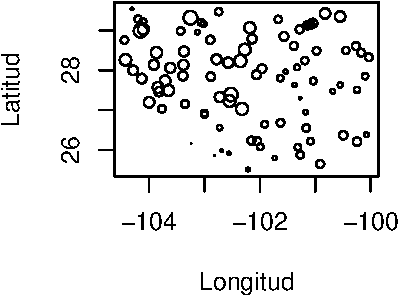
\includegraphics{Usos-Moran_files/figure-beamer/unnamed-chunk-1-1} \end{center}
\end{frame}

\begin{frame}[fragile]{Prueba previa de correlación}
\protect\hypertarget{prueba-previa-de-correlaciuxf3n}{}
\begin{Shaded}
\begin{Highlighting}[]
\FunctionTok{library}\NormalTok{(spdep)}

\NormalTok{vecindad }\OtherTok{\textless{}{-}} \FunctionTok{dnearneigh}\NormalTok{(}\AttributeTok{x =} \FunctionTok{as.matrix}\NormalTok{(datos[, }\FunctionTok{c}\NormalTok{(}\StringTok{"Longitud"}\NormalTok{, }\StringTok{"Latitud"}\NormalTok{)]), }\AttributeTok{d1 =} \DecValTok{0}\NormalTok{, }\AttributeTok{d2 =} \DecValTok{75}\NormalTok{, }\AttributeTok{longlat =}\NormalTok{ T)}
\NormalTok{vec.listw }\OtherTok{\textless{}{-}} \FunctionTok{nb2listw}\NormalTok{(vecindad)}
\NormalTok{S0 }\OtherTok{\textless{}{-}} \FunctionTok{sum}\NormalTok{(}\FunctionTok{nb2mat}\NormalTok{(vecindad))}

\NormalTok{I.meds }\OtherTok{\textless{}{-}} \FunctionTok{moran.test}\NormalTok{(}\AttributeTok{x =}\NormalTok{ datos}\SpecialCharTok{$}\NormalTok{Mediciones, }\AttributeTok{listw =}\NormalTok{ vec.listw)}
\end{Highlighting}
\end{Shaded}
\end{frame}

\begin{frame}[fragile]{Correlación espacial de mediciones}
\protect\hypertarget{correlaciuxf3n-espacial-de-mediciones}{}
\begin{Shaded}
\begin{Highlighting}[]
\NormalTok{I.meds}
\end{Highlighting}
\end{Shaded}

\begin{verbatim}
## 
##  Moran I test under randomisation
## 
## data:  datos$Mediciones  
## weights: vec.listw    
## 
## Moran I statistic standard deviate = 14.18, p-value < 2.2e-16
## alternative hypothesis: greater
## sample estimates:
## Moran I statistic       Expectation          Variance 
##       0.769152627      -0.010101010       0.003020113
\end{verbatim}
\end{frame}

\begin{frame}[fragile]{Importación de variables raster}
\protect\hypertarget{importaciuxf3n-de-variables-raster}{}
\begin{Shaded}
\begin{Highlighting}[]
\FunctionTok{library}\NormalTok{(raster)}
\NormalTok{r }\OtherTok{\textless{}{-}} \FunctionTok{stack}\NormalTok{(}\FunctionTok{paste0}\NormalTok{(}\StringTok{"../Datos{-}ejemplos/Var{-}"}\NormalTok{, }\FunctionTok{c}\NormalTok{(}\DecValTok{1}\NormalTok{, }\DecValTok{2}\NormalTok{), }\StringTok{".tif"}\NormalTok{))}
\end{Highlighting}
\end{Shaded}
\end{frame}

\begin{frame}{Importación de variables raster}
\protect\hypertarget{importaciuxf3n-de-variables-raster-1}{}
\begin{center}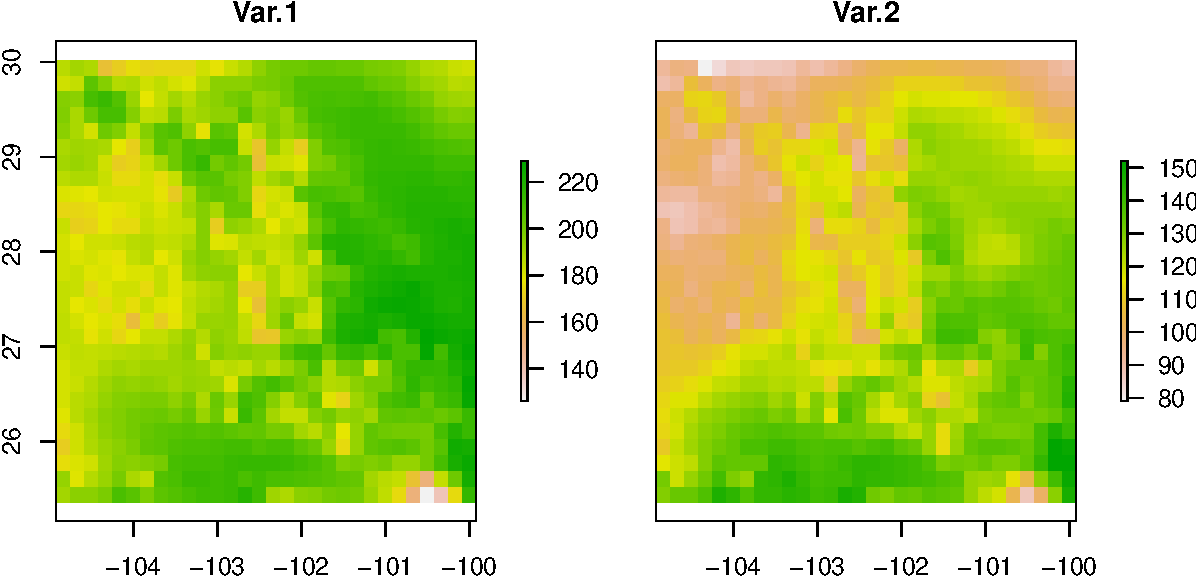
\includegraphics{Usos-Moran_files/figure-beamer/unnamed-chunk-5-1} \end{center}
\end{frame}

\begin{frame}[fragile]{Extracción de valores en localidades de muestreo}
\protect\hypertarget{extracciuxf3n-de-valores-en-localidades-de-muestreo}{}
\begin{Shaded}
\begin{Highlighting}[]
\NormalTok{r.extract }\OtherTok{\textless{}{-}} \FunctionTok{data.frame}\NormalTok{(}\FunctionTok{extract}\NormalTok{(r, datos[, }\FunctionTok{c}\NormalTok{(}\StringTok{"Longitud"}\NormalTok{, }\StringTok{"Latitud"}\NormalTok{)]))}
\NormalTok{datos }\OtherTok{\textless{}{-}} \FunctionTok{data.frame}\NormalTok{(datos, r.extract)}
\end{Highlighting}
\end{Shaded}

\begin{longtable}[]{@{}rrrrr@{}}
\toprule()
Longitud & Latitud & Mediciones & Var.1 & Var.2 \\
\midrule()
\endhead
-103.3797 & 28.13648 & 4.462367 & 188 & 108 \\
-104.1984 & 29.28437 & 3.245952 & 197 & 106 \\
-102.5610 & 25.91724 & 1.421369 & 208 & 136 \\
-101.2730 & 27.30093 & 1.112655 & 221 & 137 \\
-104.4254 & 28.26304 & 5.107742 & 173 & 89 \\
-101.0895 & 29.13997 & 3.628602 & 214 & 125 \\
\bottomrule()
\end{longtable}
\end{frame}

\begin{frame}[fragile]{Ajuste de primer modelo}
\protect\hypertarget{ajuste-de-primer-modelo}{}
\begin{Shaded}
\begin{Highlighting}[]
\NormalTok{modelo}\FloatTok{.1} \OtherTok{\textless{}{-}} \FunctionTok{lm}\NormalTok{(Mediciones }\SpecialCharTok{\textasciitilde{}}\NormalTok{ Var}\FloatTok{.2}\NormalTok{, }\AttributeTok{data =}\NormalTok{ datos)}
\FunctionTok{summary}\NormalTok{(modelo}\FloatTok{.1}\NormalTok{)}
\end{Highlighting}
\end{Shaded}

\begin{verbatim}
## 
## Call:
## lm(formula = Mediciones ~ Var.2, data = datos)
## 
## Residuals:
##     Min      1Q  Median      3Q     Max 
## -3.5996 -0.5276  0.2858  0.8551  1.9831 
## 
## Coefficients:
##              Estimate Std. Error t value Pr(>|t|)    
## (Intercept) 15.120815   1.115281   13.56   <2e-16 ***
## Var.2       -0.100829   0.009265  -10.88   <2e-16 ***
## ---
## Signif. codes:  0 '***' 0.001 '**' 0.01 '*' 0.05 '.' 0.1 ' ' 1
## 
## Residual standard error: 1.216 on 98 degrees of freedom
## Multiple R-squared:  0.5472, Adjusted R-squared:  0.5426 
## F-statistic: 118.4 on 1 and 98 DF,  p-value: < 2.2e-16
\end{verbatim}
\end{frame}

\begin{frame}[fragile]{Extracción y visualización de residuales}
\protect\hypertarget{extracciuxf3n-y-visualizaciuxf3n-de-residuales}{}
\begin{Shaded}
\begin{Highlighting}[]
\NormalTok{datos}\SpecialCharTok{$}\NormalTok{Residuales }\OtherTok{\textless{}{-}}  \FunctionTok{residuals}\NormalTok{(modelo}\FloatTok{.1}\NormalTok{)}
\FunctionTok{with}\NormalTok{(datos, }\FunctionTok{plot}\NormalTok{(Longitud, Latitud, }\AttributeTok{cex =}\NormalTok{ Residuales))}
\end{Highlighting}
\end{Shaded}

\begin{center}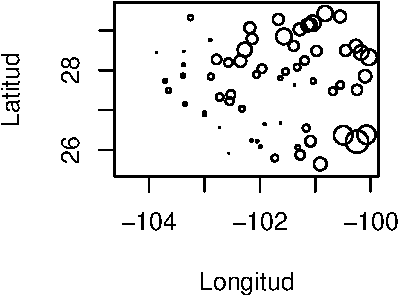
\includegraphics{Usos-Moran_files/figure-beamer/unnamed-chunk-9-1} \end{center}
\end{frame}

\begin{frame}[fragile]{Prueba de correlación de residuales}
\protect\hypertarget{prueba-de-correlaciuxf3n-de-residuales}{}
\begin{Shaded}
\begin{Highlighting}[]
\NormalTok{I.res }\OtherTok{\textless{}{-}} \FunctionTok{moran.test}\NormalTok{(}\AttributeTok{x =}\NormalTok{ datos}\SpecialCharTok{$}\NormalTok{Residuales, }\AttributeTok{listw =}\NormalTok{ vec.listw)}
\NormalTok{I.res}
\end{Highlighting}
\end{Shaded}

\begin{verbatim}
## 
##  Moran I test under randomisation
## 
## data:  datos$Residuales  
## weights: vec.listw    
## 
## Moran I statistic standard deviate = 15.7, p-value < 2.2e-16
## alternative hypothesis: greater
## sample estimates:
## Moran I statistic       Expectation          Variance 
##       0.852139315      -0.010101010       0.003016244
\end{verbatim}
\end{frame}

\end{document}
